
%%%%%%%%%%%%%%%%%%%%%%%%%%%%%%%%%%%%%%%%%%%%%%%%%%%%%%%%%%%%%%%%%%%%%%%%%%%%%%%
%     STYLE POUR LES EXPOSÉS TECHNIQUES 
%         3e année INSA de Rennes
%
%             NE PAS MODIFIER
%%%%%%%%%%%%%%%%%%%%%%%%%%%%%%%%%%%%%%%%%%%%%%%%%%%%%%%%%%%%%%%%%%%%%%%%%%%%%%%

\documentclass[a4paper,11pt]{report}
\usepackage[dvips]{graphicx}
\usepackage[T1]{fontenc}
\usepackage[utf8]{inputenc}
\usepackage[french]{babel}
\usepackage{lmodern} \normalfont
\DeclareFontShape{T1}{lmr}{bx}{sc}{<-> ssub * cmr/bx/sc}{}
\usepackage{textcomp}
\usepackage{fixltx2e}
\usepackage{exptech} % inclusion du style immposé
\usepackage{amsmath}
\usepackage{amssymb}
\usepackage{graphicx}
\usepackage{wrapfig}
\usepackage{subcaption}
\usepackage{listings}
\usepackage{color}
\usepackage{pdfpages}
\usepackage[colorlinks=true,
			linkcolor=blue,
			bookmarksnumbered=true,
			pdftitle={Report},
			pdfauthor={Julien B.},
			pdfborder={0 0 0},
			pdfsubject={mittelwerk}]{hyperref}


\title{\textbf{Contrôleurs dans l'espace}}
\author{Julien \textsc{Bouvet}, Antoine \textsc{Chenon}, Mikaïl \textsc{Demirdelen}, Hoel \textsc{Kervadec}
        \\
        Encadrants : Yann \textsc{Ricquebourg}, Loic \textsc{Helouet}}
\date{Juin 2014}
\markright{Contrôleurs dans l'espace}


\thispagestyle{empty}

%%%%%%%%%%%%%%%%%%%%%%%%%%%%%%%%%%%%%%%%%%%%%%%%%%%%%%%%%%%%%%%%%%%%%%%%%%%%%%%

\begin{document}          

\maketitle                
\part{Avant-propos}

\begin{figure}[!h]
            \begin{center}
                
\includegraphics[width=0.7\textwidth]{img/orbiter_logo.png}
            \end{center}
\end{figure}

\section{Un simulateur en temps réel}

Orbiter est un simulateur de vol spatial, créé par Dr. Martin Schweiger en 2000 et ce afin de combler le manque de simulateur de vol réaliste disponible sur internet. Gratuit mais non libre, un kit de développement a fait son apparition pour permettre à tout un chacun de développer son propre vaisseau. Fourni avec un lot de scénarios et de vaisseaux, Orbiter permet d'expérimenter et de mieux appréhender les lois de la physique.

C'est dans cette optique que nous proposons une première démarche d'automatisations des vaisseaux dans Orbiter.

Dans un premier temps ce projet est compatible avec un seul vaisseau : le Shuttle A.

\section{Module lunaire}

Le Shuttle A est un module lunaire : en effet il est conçu pour permettre aux spationautes de rentrer sur Terre une fois l'alunissage terminé. Ces caractéristiques sont donc plus adaptées à cet environnement. En effet le décollage depuis la Terre est plus diffcile (compte tenu de la gravité, plus forte que sur la Lune) et plus gourmand en carburant. Cependant le Shuttle A a deux avantages :

\begin{itemize}
	\item Il dispose de nombreux propulseurs, ce qui en facilite la manoeuvre
	\item Il est codé en une seule classe C++ :, c'est transparent pour l'utilisateur, mais dans le cas de notre travail, cela simplifier grandement l'étude.
\end{itemize}


\section{Théorie du contrôle}
Pour pouvoir automatiser le pilotage des vaisseau, en particulier du ShuttleA nous disposons de plusieurs outils formels, dont la théorie du contrôle.

C'est un moyen de formaliser le fait qu'un système, pour se maintenir sur une trajectoire prend des mesures, les compare à des références et corrige si nécessaire. C'est une boucle qui va des capteurs vers le contrôleur, chargé de prendre les décisions pour suivre l'objectif.

\begin{figure}[!h]
            \begin{center}
                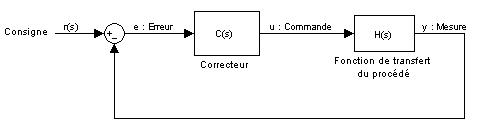
\includegraphics[width=0.7\textwidth]{img/boucle_controle.jpg}
            \end{center}
\end{figure}

\section{Automates}
Les automates sont un ensemble d'états et de transitions, qui correspondent à des états d'un système. Par exemple on peut imaginer qu'une lampe soit modélisée par un automate. Elle aurait deux états : Allumée, éteinte. Cette lampe peut passer d'un état à l'autre grâce à des transitions.
Ces transitions définissent sous quelles conditions le système change d'état.
Pour la lampe, la transition de l'état éteinte vers allumée se fait par exemple si elle est alimentée et vice-versa.

\begin{figure}[!h]
            \begin{center}
                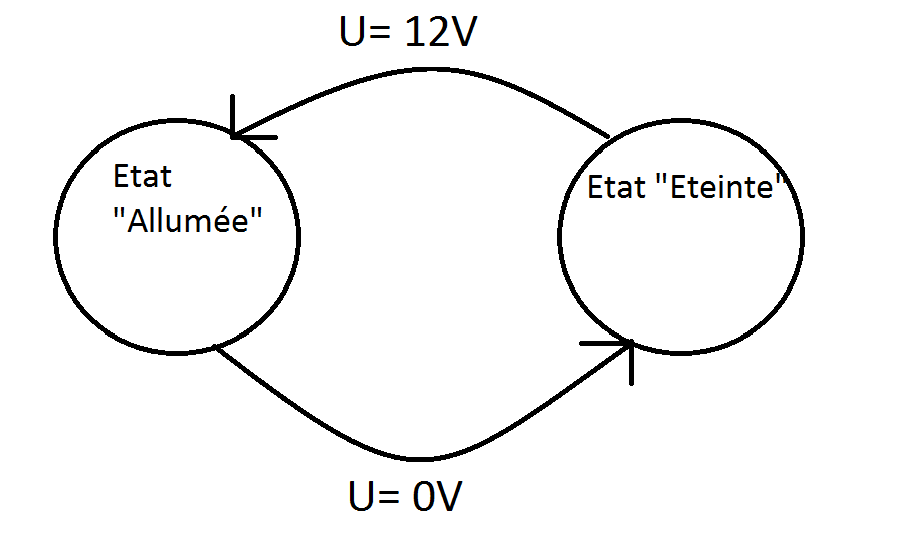
\includegraphics[width=0.7\textwidth]{img/automatelas.png}
            \end{center}
\end{figure}

Pour le vaisseau on peut imaginer une infinité d'états différents, ce qui permet de contrôler le vaisseau à notre guise. Par exemple l'état "`Propulsion MAXI"' avec une transition sur l'état "`Propulsion Gauche seule"' en cas de détection d'obstacle.

\part{Langage Mittlewerk}

\section{Introduction}
Nous avons créé un langage simple permettant de piloter le vaisseau sans maîtriser le C++. En effet, ce langage permet de créer facilement des automates, et donc de créer un contrôleur personnalisé.
Certains aspects du langage sont proches du C++ mais ce sont des concepts classiques en programmation (affectation, déclaration ...).

\section{Instructions basiques}
Toutes les instructions se terminent par un ';' pour indiquer au compilateur qu'une instruction est complète.

\subsection{Variables}
Une variable a un nom et un type, il faut donc les déclarer au compilateur avant de pouvoir les utiliser. Cela se fait très simplement : 
\begin{center}
\texttt{type nom;}
\end{center}
Par exemple, si vous souhaitez définir un double (nombre à virgule à valeur max très élevée) que vous appelez toto, il vous faudra avant de l'avoir utilisé l'avoir défini de cette façon : 
\begin{center}
\texttt{DOUBLE toto;}
\end{center}
Pour affecter une valeur, la démarche est identique à la plupart des langages :
\begin{center}
	\texttt{toto = 42;}
	
	\texttt{toto = toto + 1;}
	
	\texttt{toto = max(1, toto);}
\end{center}
On peut affecter à une variable la valeur de retour d'une fonction, d'une autre variable ... Il faut juste vérifier que le type que l'on donne à la variable correspond à celui qu'on lui a donné lors de sa déclaration.

\subsection{Fonctions}
Les fonctions peuvent être déclarées, hors du corps d'une fonction, et être appelées, dans le corps d'une fonction ou dans un etat de l'Automate.

Pour déclarer une fonction c'est très simple : 
\begin{center}
\texttt{type nomDeFonction(type1 Param1, type2 Param2 ...) \{ corps de la fonction \}}
\end{center}

Si la fonction a un type différent de VOID, elle doit retourner une valeur : 
\begin{center}
\texttt{RETURN toto;}
\end{center}

Pour l'appeler : \texttt{ nomDeFonction(param1, param2, ...)}

\subsection{Commentaires}
Il est parfois très utile de commenter son code : ce qui est commenté n'est pas interpreté lors de la compilation, ce ne sont que des informations pour les humains.
Pour encadrer du commentaire il faut mettre /* avant le commentaire, */ à la fin.
\begin{center}
\texttt{VOID fonctionInutile() \{ /* cette fonction ne fait rien*/ \}}
\end{center}

\subsubsection{Exemple de synthèse:}

\texttt{DOUBLE megaBadAss(DOUBLE toto) \{}

\texttt{	goToSchool(toto); /* Fonction fictive, rassurez vous ;) */}

\texttt{	RETURN 42;}

\texttt{\}}


\end{document}




%%%%%%%%%%%%%%%%%%%%%%%%%%%%%%%%%%%%%%%%%%%%%%%%%%%%%%%%%%%%%%%%%%%%%%%%%%%%%%%
